\documentclass{article}

\usepackage{graphicx}
\usepackage{tikz}
\usepackage{tikzsymbols}
\usetikzlibrary{calc,patterns,shapes.geometric}
\pagestyle{empty}
\usepackage[margin=0pt]{geometry}
\geometry{papersize={14in,12in}}

\def\centerarc[#1](#2)(#3:#4:#5){\draw[#1] ($(#2)+({#5*cos(#3)},{#5*sin(#3)})$) arc (#3:#4:#5);}

\begin{document}
	\begin{figure}
		\centering
		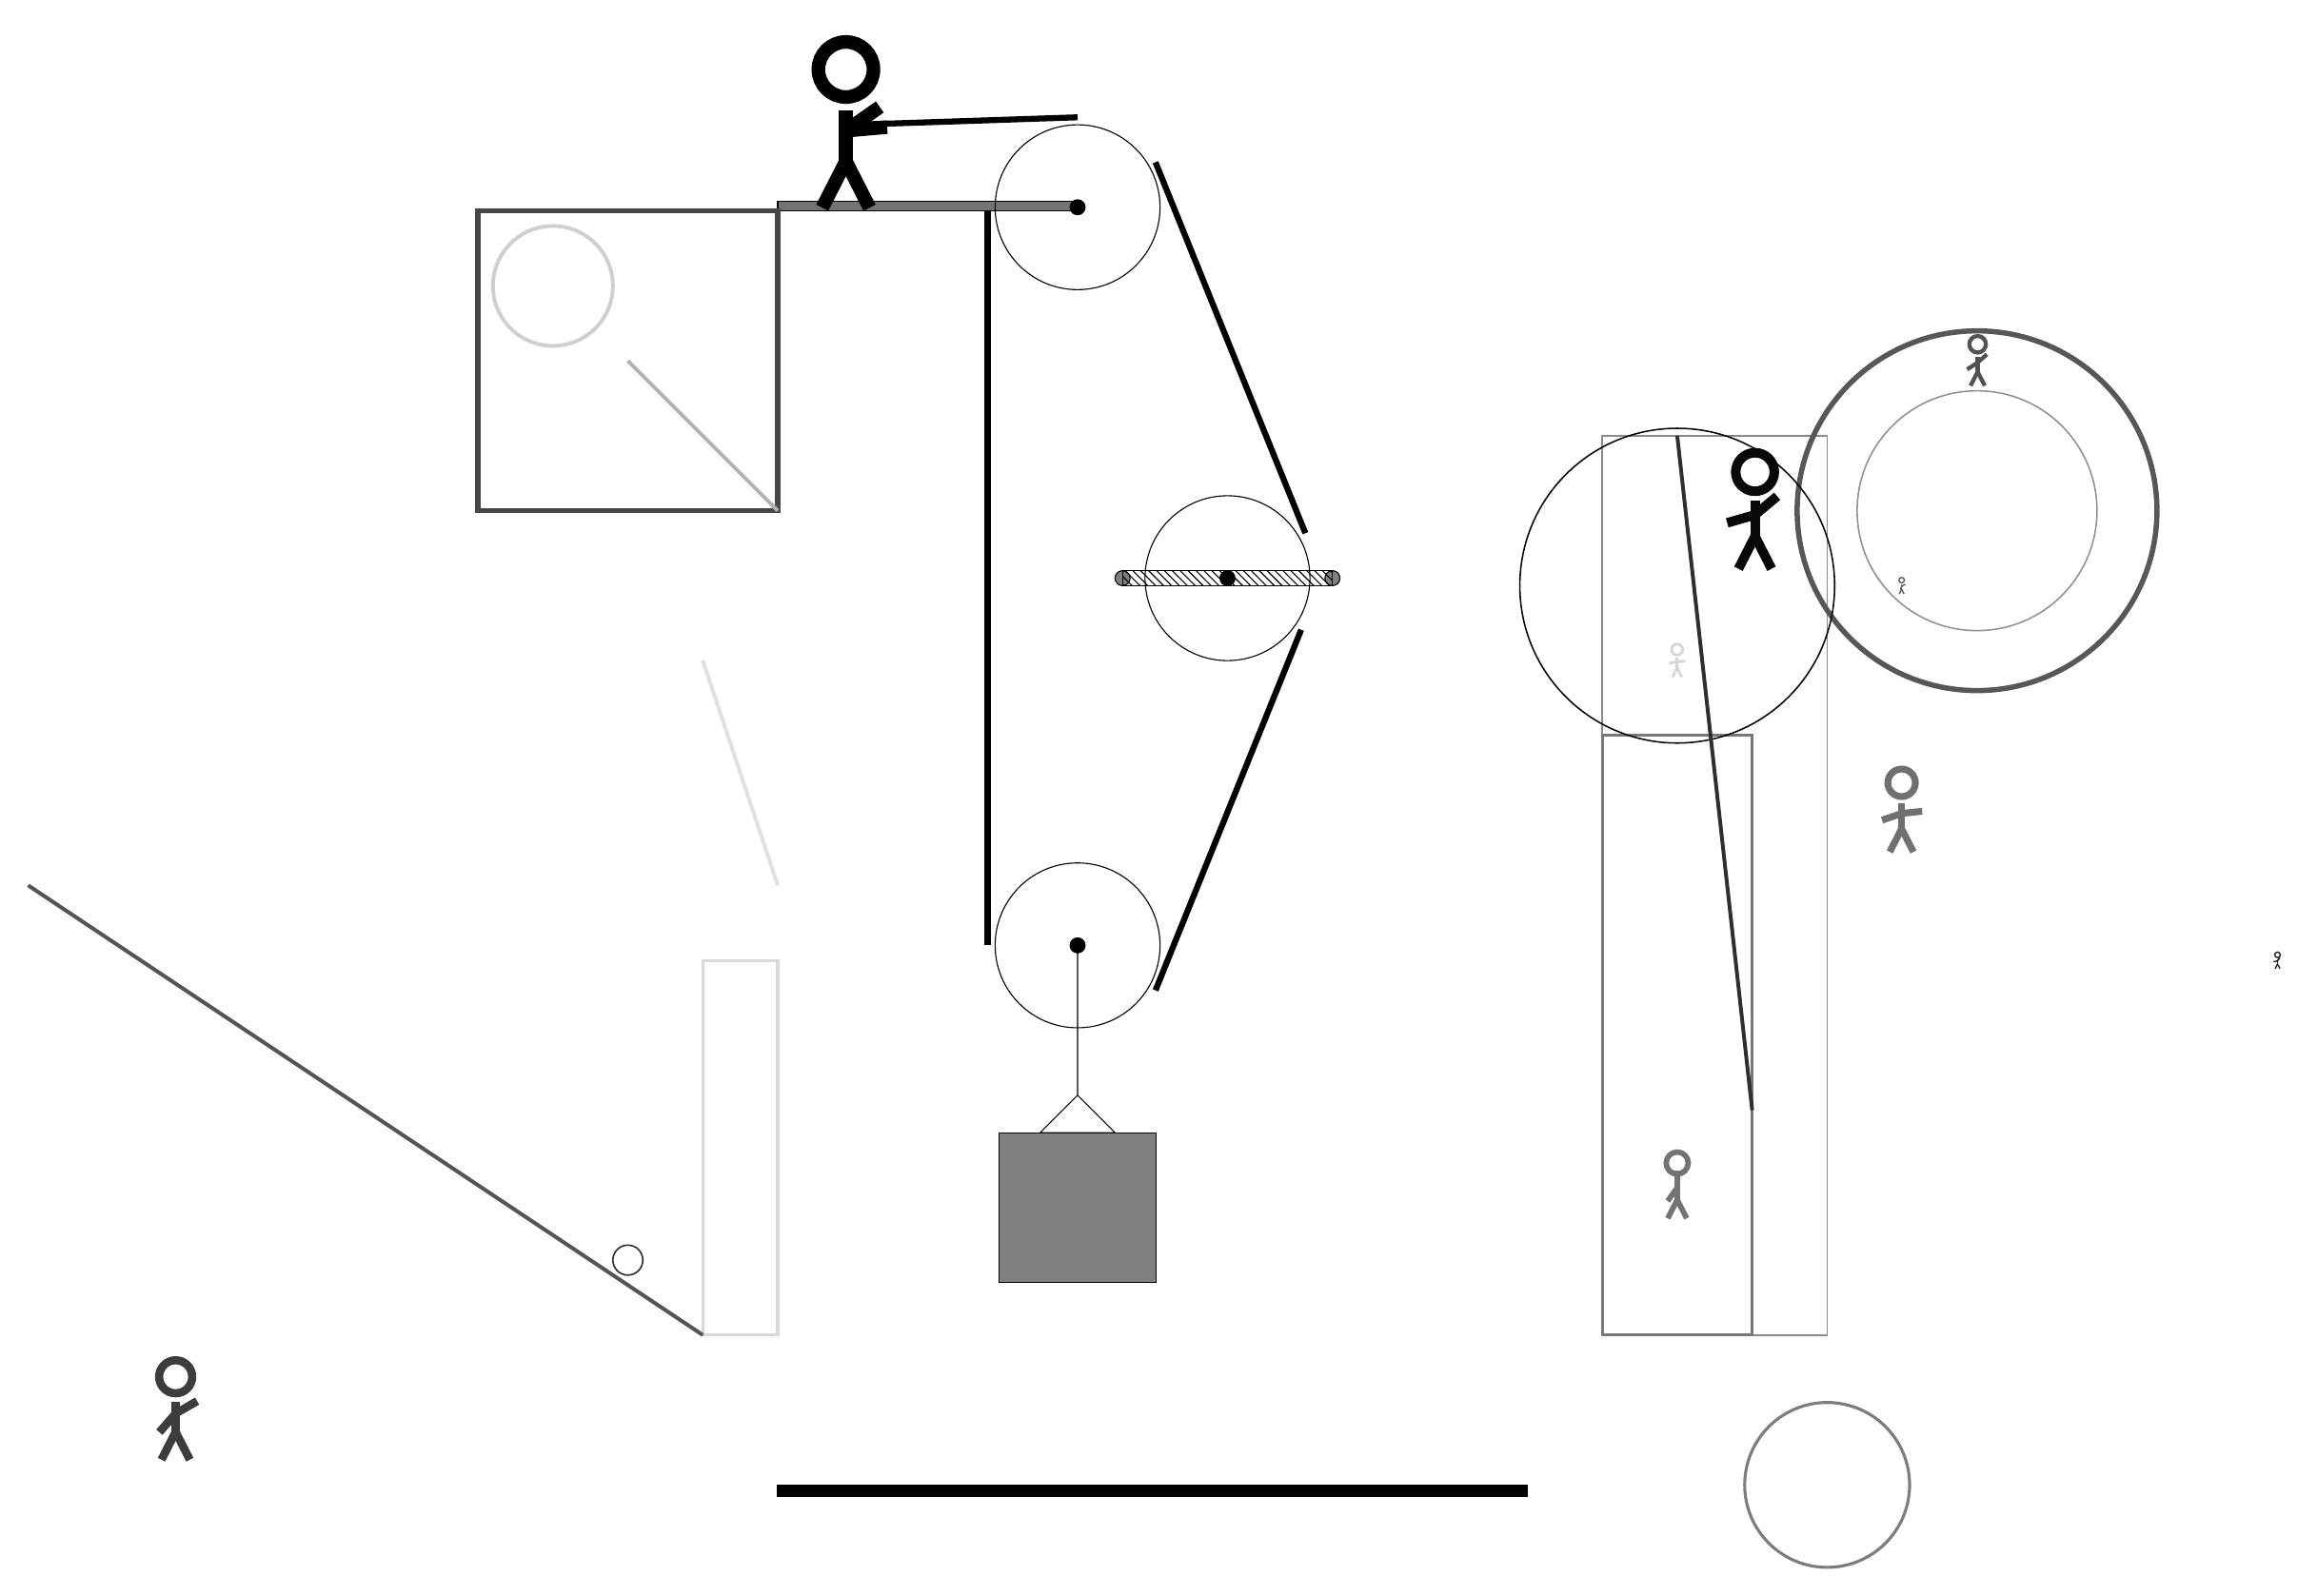
\begin{tikzpicture}
			%%%%% START %%%%%
			
			\draw[fill=black!55] (-2, 14) rectangle (2, 14.125);
			
			\draw (2, 4.2) circle (1.1);
			\draw[fill=black] (2, 4.2) circle (0.1);
			
			\draw (2, 14.05) circle (1.1);
			\draw[fill=black] (2, 14.05) circle (0.1);
			
			\draw[line width=0.5mm, color=black!12](-3, 8) -- (-2, 5);
			
			\draw [line width=0.2mm, color=black!43](14, 10) circle (1.6);
			\node[line width=0.3mm, color=black!76] at (-10, -2) {\Strichmaxerl[6][49][30]};
			\draw[line width=0.4mm, color=black!15] (-3, 4) rectangle (-2, -1);
			\node[line width=0.7mm, color=black!55] at (10, 1) {\Strichmaxerl[4][55][90]};
			\draw[line width=0.5mm, color=black!67](-3, -1) -- (-12, 5);
			\draw [line width=0.5mm, color=black!19](-5, 13) circle (0.8);
			
			\draw[line width=0.2mm, color=black!46] (9, -1) rectangle (12, 11);
			\draw[line width=0.4mm, color=black!53] (9, 7) rectangle (11, -1);
			\node[line width=0.7mm, color=black!97] at (11, 10) {\Strichmaxerl[7][16][40]};
			\draw[line width=0.7mm, color=black!72] (-2, 10) rectangle (-6, 14);
			\node[line width=0.5mm, color=black!85] at (18, 4) {\Strichmaxerl[1][11][55]};
			\draw [line width=0.7mm, color=black!66](14, 10) circle (2.4);
			
			\node[line width=0.4mm, color=black!68] at (14, 12) {\Strichmaxerl[3][33][42]};
			\node[line width=0.3mm, color=black!16] at (10, 8) {\Strichmaxerl[2][11][5]};
			\draw [line width=0.2mm, color=black!83](-4, 0) circle (0.2);
			
			\draw [line width=0.4mm, color=black!51](12, -3) circle (1.1);
			
			\node[line width=0.6mm, color=black!63] at (13, 9) {\Strichmaxerl[1][73][28]};
			\draw [line width=0.2mm, color=black!97](10, 9) circle (2.1);
			
			\draw[line width=0.5mm, color=black!30](-2, 10) -- (-4, 12);
			\draw[line width=0.5mm, color=black!82](11, 2) -- (10, 11);
			
			\node[line width=0.7mm, color=black!56] at (13, 6) {\Strichmaxerl[5][19][6]};
			
			
			\draw[fill=white](4, 9.1) circle (1.1);
			\draw[fill=black] (4, 9.1) circle (0.1);
			\draw[fill=black!50] (2.6, 9.1) circle (0.1);
			\draw[fill=black!50] (5.4, 9.1) circle (0.1);
			\draw[pattern=north west lines, pattern color=black] (2.6, 9.2) rectangle (5.4, 9.0);
			
			\draw (2, 4.2) -- (2, 2.2) -- (1.5, 1.7) -- (2.5, 1.7) -- (2, 2.2);
			\draw[fill=black!50] (0.95, 1.7) rectangle (3.05, -0.3);
			
			\draw[line width=0.8mm] (0.8, 14) -- (0.8, 4.2);
			\centerarc[line width=0.8mm](2, 4.2)(180:330:1.2000000000000002);
			\draw[line width=0.8mm](3.0392, 3.6) -- (4.983, 8.4117);
			\centerarc[line width=0.8mm](4, 9.1)(390:325:1.2000000000000002);
			\draw[line width=0.8mm](5.0392, 9.7) -- (3.0392, 14.65);
			\centerarc[line width=0.8mm](2, 14.05)(30:90:1.2000000000000002);
			\draw[line width=0.8mm](2, 15.25) -- (-1, 15.15);
			
			\node at (-1, 15.15) {\Strichmaxerl[10][-175][35]};
			
			\draw[fill=black] (-2, -3) rectangle (8, -3.15);
			
			%%%%% END %%%%%
		\end{tikzpicture}
	\end{figure}	
\end{document}